\break

\hypertarget{biosketches}{%
\section*{Biosketches}\label{biosketches}}
\addcontentsline{toc}{section}{Biosketches}

\textbf{Ruan van Mazijk} is a Masters student broadly interested in
comparative biology and \ldots{}

\textbf{Michael D. Cramer}

\textbf{G. Anthony Verboom}

\hypertarget{author-contributions}{%
\section*{Author contributions}\label{author-contributions}}
\addcontentsline{toc}{section}{Author contributions}

MDC and GAV conceived the study question, which RVM investigated under
their supervision for his BSc Hons project. The analyses and programming
work were largely devised by RVM, with input from the other authors, and
was carried out by RVM. RVM wrote the first draft of the manuscript and
all authors contributed equally thereafter.

\hypertarget{orcid-numbers}{%
\section*{ORCID numbers}\label{orcid-numbers}}
\addcontentsline{toc}{section}{ORCID numbers}

RVM: 0000-0003-2659-6909

MDC: 0000-0003-0989-3266

GAV: 0000-0002-1363-9781

\break

\hypertarget{tables}{%
\section*{Tables}\label{tables}}
\addcontentsline{toc}{section}{Tables}

\begin{longtable}[]{@{}lll@{}}
\caption{(ref:data-sources)}\tabularnewline
\toprule
Variable & Source (Dataset code) & Citation\tabularnewline
\midrule
\endfirsthead
\toprule
Variable & Source (Dataset code) & Citation\tabularnewline
\midrule
\endhead
Elevation & SRTM v2.0 & @Farr2007\tabularnewline
NDVI & MODIS (MOD13C2) & @MOD13C2\tabularnewline
\textbf{Climatic variables} & NA & NA\tabularnewline
Surface T & MODIS (MOD11C3) & @MOD11C3\tabularnewline
MAP & CHIRPS v2.0 & @Funk2015\tabularnewline
PDQ & CHIRPS v2.0 & @Funk2015\tabularnewline
\textbf{Edaphic variables} & SoilGrids250m & @Hengl2017\tabularnewline
pH & PHIKCL\_M\_250m & NA\tabularnewline
CEC & CECSOL\_M\_250m & NA\tabularnewline
Soil C & OCDENS\_M\_250m & NA\tabularnewline
Clay & CLYPPT\_M\_250m & NA\tabularnewline
Plant species occurrence & GBIF & @GBIFCape, @GBIFSWA\tabularnewline
\bottomrule
\end{longtable}

(ref:data-sources) Data sources used in this study. Abbreviations are as
follows:.

\begin{table}[!h]
\caption{\label{tab:turnover-vs-geodist-model-table}(ref:turnover-vs-geodist-model-table)}

\centering
\begin{tabular}[t]{lrl}
\toprule
Term & Estimate & $P$-value\\
\midrule
Intercept & -0.311 & < 0.001\\
log Distance between cells & 0.093 & < 0.001\\
Cape & 0.388 & < 0.001\\
log Distance between cells $\times$ Cape & -0.026 & < 0.001\\
\bottomrule
\end{tabular}
\end{table}

(ref:turnover-vs-geodist-model-table) Estimated coefficients and
significances (\(P\)-value) following quantile regression of the
5\%-quantile (\(\tau = 0.05\)) of pairwise species turnover (as Jaccards
distance) as a function of the geographic distance (km, log-transformed)
between QDS cells. The Cape term represents the difference between Cape
and SWA species turnover, for a given geographic distance.

\begin{table}[!h]
\caption{\label{tab:species-model-table}(ref:species-model-table)}

\centering
\begin{tabular}[t]{lrr}
\toprule
Term & Estimate & $P$-value\\
\midrule
Intercept & -3062.297 & 0.000\\
$log(\overline{S_{QDS}} + 1)$ & 595.574 & 0.000\\
$\overline{J_{QDS}}$ & 338.589 & 0.534\\
$SWA$ & 2905.604 & 0.001\\
$log(\overline{S_{QDS}} + 1) \times SWA$ & -333.908 & 0.000\\
$\overline{J_{QDS}} \times SWA$ & -1246.109 & 0.073\\
\bottomrule
\end{tabular}
\end{table}

(ref:species-model-table) Estimated coefficients and significances
(\(P\)-value) following multiple linear regression of HDS species
richness (\(S_{HDS}\)) against the mean QDS species richness
(\(\overline{S_{QDS}}\)) and turnover (\(\overline{J_{QDS}}\); Jaccards
distance) within a given HDS, of the form in Equation
@ref(eq:S-HDS-formula). The Cape was fit as the baseline, hence SWA
represents the categorical term here. This was model was better fitting
than a similar model without a region category (\(\Delta AIC =\) 90.56).
Note, this model does not represent those curves plot in Figures
@ref(fig:richness-vs-turnover) and @ref(fig:richness-vs-turnover-3QDS)
(there, the curves are from simple linear regressions of the variables
in each panel, separated by region).

\begin{table}[!h]

\caption{\label{tab:species-roughness-AICc}(ref:species-roughness-AICc)}
\centering
\begin{tabular}[t]{lrrr}
\toprule
Model predictors & $AICc$ & $\Delta AICc$ & $w_{AICc}$\\
\midrule
\addlinespace[0.3em]
\multicolumn{4}{l}{\textbf{Cape:}}\\
\hspace{1em}Absolute variables & 2112.49 & 0.00 & 1.00\\
\hspace{1em}Non-elevation variables & 2179.35 & 66.86 & 0.00\\
\hspace{1em}All & 2192.59 & 80.10 & 0.00\\
\hspace{1em}Soil variables & 2197.76 & 85.28 & 0.00\\
\hspace{1em}Roughness variables & 2208.43 & 95.94 & 0.00\\
\hspace{1em}Non-soil variables & 2218.08 & 105.59 & 0.00\\
\hspace{1em}Elevation & 2267.30 & 154.81 & 0.00\\
\hspace{1em}Null & 3099.37 & 986.89 & 0.00\\
\addlinespace[0.3em]
\multicolumn{4}{l}{\textbf{SWA:}}\\
\hspace{1em}Absolute variables & 826.47 & 0.00 & 0.69\\
\hspace{1em}Non-elevation variables & 828.29 & 1.82 & 0.28\\
\hspace{1em}All & 833.44 & 6.97 & 0.02\\
\hspace{1em}Soil variables & 835.92 & 9.45 & 0.01\\
\hspace{1em}Non-soil variables & 848.57 & 22.11 & 0.00\\
\hspace{1em}Roughness variables & 868.89 & 42.42 & 0.00\\
\hspace{1em}Elevation & 970.19 & 143.73 & 0.00\\
\hspace{1em}Null & 27172.21 & 26345.74 & 0.00\\
\addlinespace[0.3em]
\multicolumn{4}{l}{\textbf{Both:}}\\
\hspace{1em}Absolute variables & 1286.27 & 0.00 & 1.00\\
\hspace{1em}Roughness variables & 1338.16 & 51.89 & 0.00\\
\hspace{1em}Non-elevation variables & 1364.26 & 77.98 & 0.00\\
\hspace{1em}Elevation & 1371.30 & 85.02 & 0.00\\
\hspace{1em}Soil variables & 1371.47 & 85.19 & 0.00\\
\hspace{1em}Non-soil variables & 1380.38 & 94.11 & 0.00\\
\hspace{1em}All & 1390.78 & 104.50 & 0.00\\
\hspace{1em}Null & 1404.05 & 117.78 & 0.00\\
\bottomrule
\end{tabular}
\end{table}

(ref:species-roughness-AICc) Comparisons of Akaike information criterion
values (small sample-size-corrected, \(AICc\)) of various geographically
weighted regressions (GWR) of log-transformed species richness as a
function of various sets of environmental variables. Models were fit for
the Cape and SWA richness and environmental data both separately and
together. GWR methods preclude the need for a categorical predictor for
the Cape vs SWA, as the longitudinal (and to a lesser extent
latitudinal) differences between the regions allows local regression
coefficients in each region to differ.

\break

\hypertarget{figure-captions}{%
\section*{Figure captions}\label{figure-captions}}
\addcontentsline{toc}{section}{Figure captions}

Captions are also repeated alongside their respective figures for
readability.

\hypertarget{figure-reffigroughness}{%
\subsection*{Figure @ref(fig:roughness)}\label{figure-reffigroughness}}
\addcontentsline{toc}{subsection}{Figure @ref(fig:roughness)}

(ref:roughness) Comparisons of different types of environmental
heterogeneity in the Cape and SWA. (a) Example distributions of
roughness values (Equation @ref(eqn:roughness)), showing the different
extremes in environmental heterogeneity observed in each region when
compared at fine (0.05º) and coarse (3QDS) scales. Each distribution has
under it area 1. Distributions were constructed with Gaussian kernels,
with bandwidth following Silverman's ``rule of thumb''
{[}@Silverman1986;
\(0.9 \times min \left ( \left \{ \sigma, \frac{IQR}{1.34 \times n^{-\frac{1}{5}}} \right \} \right )\){]}.
These distributions of roughness values were compared between the Cape
and SWA at each of the four spatial scales, not just 0.05º and 3QDS,
using non-parametric Mann-Whitney \(U\)-tests to test for differences.
The ``common language effect size'' (\(CLES\), see text) describes these
differences (b). \(U\)-tests for almost all environmental variables
yielded significant differences (\(P < 0.05\)) between Cape and SWA
values (\(NS\), non-significant differences).

(ref:roughness)

\hypertarget{figure-reffigrichness-vs-turnover}{%
\subsection*{Figure
@ref(fig:richness-vs-turnover)}\label{figure-reffigrichness-vs-turnover}}
\addcontentsline{toc}{subsection}{Figure @ref(fig:richness-vs-turnover)}

(ref:richness-vs-turnover) Regressions involving plant species richness
and turnover. Species turnover (as Jaccards distance) between QDS-pairs
increases as pairs are more geographically separated (a). Species
turnover was calculated for all possible pairs of cells, but only the
turnover values for a random 5000 pairs in each region have been
plotted, for clarity. Fitted lines represent the 5\%-quantile
regressions of turnover as a function of log-distance for each region
separately. Following a 5\%-quantile regression of turnover as a
function of log-distance with region as a categorical variable (Table
@ref(tab:turnover-vs-geodist-model-table)), a significant interaction
between distance and region was found (\(P < 0.001\)), such that the
Cape positively effects the distance slope term. Scatter-plots of
HDS-scale species richness against the average QDS-scale richness in a
given HDS (b) and the average species turnover between QDS in a given
HDS (c). Curves represent simples linear regressions of HDS richness
against these two respective independent variables (note, mean QDS
richness was \(log(x + 1)\)-transformed), separately for each region,
for illustration of the two regions' differences.

(ref:richness-vs-turnover)

\hypertarget{figures}{%
\section*{Figures}\label{figures}}
\addcontentsline{toc}{section}{Figures}

\begin{figure}[H]
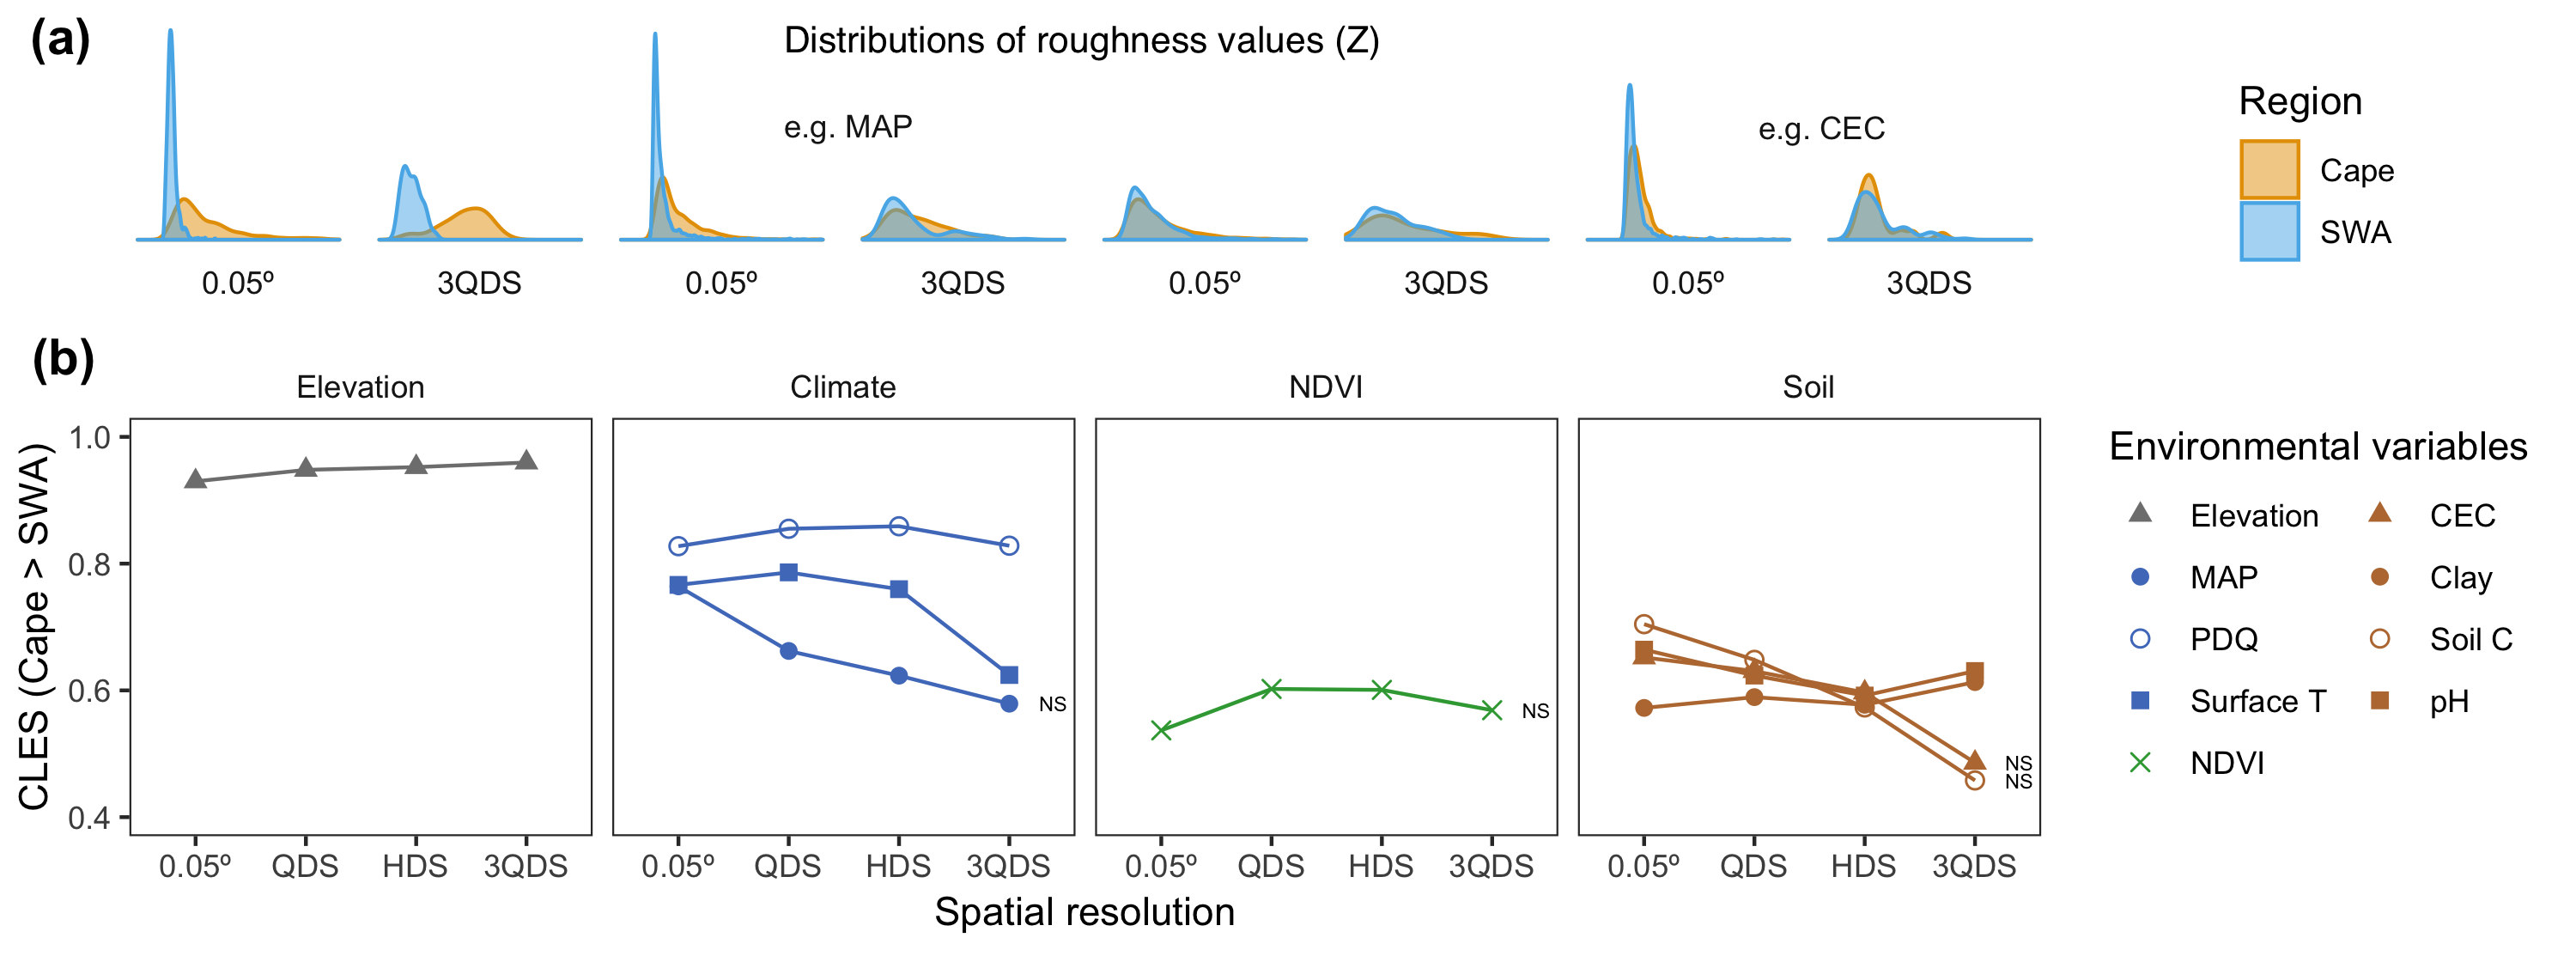
\includegraphics[width=18cm]{/Users/ruanvanmazijk/projects/Cape-vs-SWA/figures/fig-1-roughness_manual-edit} \caption{(ref:roughness)}\label{fig:roughness}
\end{figure}

\begin{figure}[H]
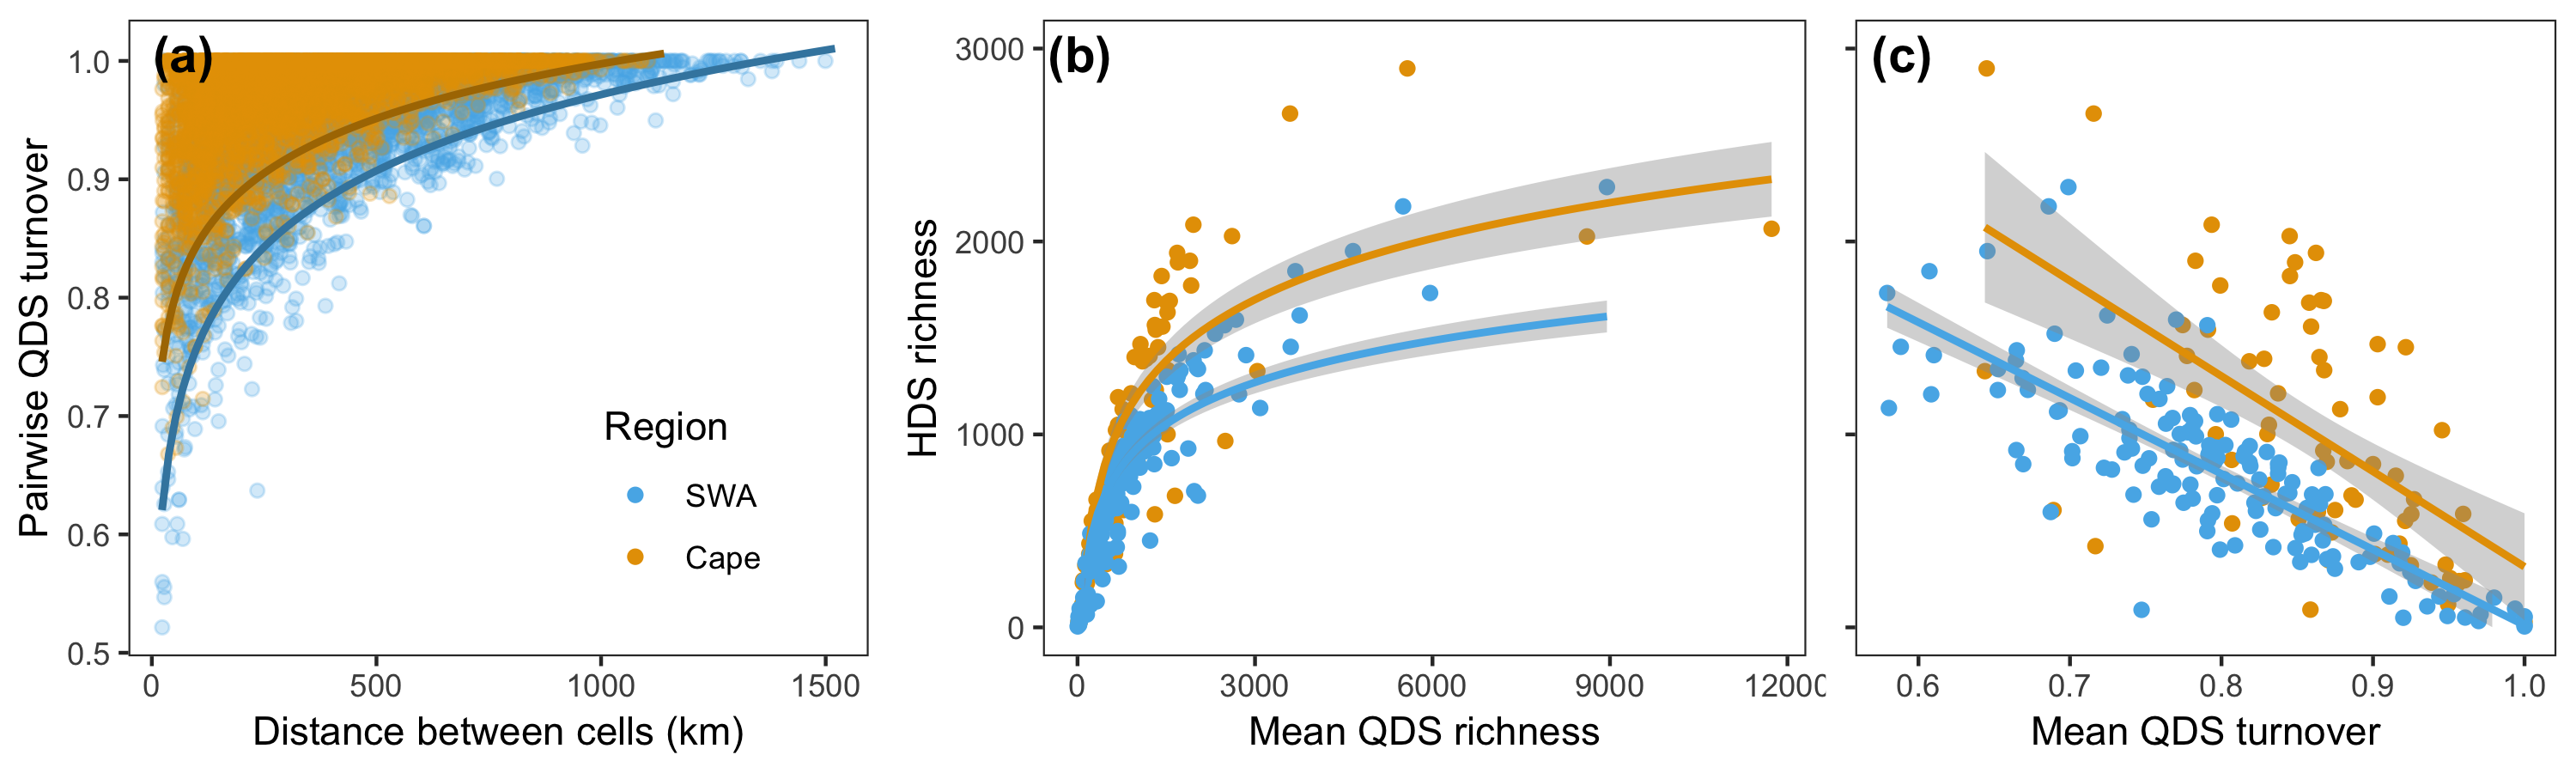
\includegraphics[width=18cm]{/Users/ruanvanmazijk/projects/Cape-vs-SWA/figures/fig-2-richness-vs-turnover} \caption{(ref:richness-vs-turnover)}\label{fig:richness-vs-turnover}
\end{figure}
